\documentclass[10pt]{beamer}
\usetheme{Montpellier}

\usepackage{xspace, alltt}

\newcommand{\TODO}[2][]{[\textcolor{red}{TODO (#1):} \emph{#2}]}
\newcommand{\coq}{Coq\xspace}
\newcommand{\coqdoc}{Coqdoc\xspace}
\newcommand{\coqmakefile}{\texttt{coq\_makefile}\xspace}
\newcommand{\community}{Coq-community\xspace}
\newcommand{\gaia}{Gaia\xspace}
\newcommand{\alectr}{Alectryon\xspace}
\newcommand{\equations}{Equations\xspace}
\newcommand{\Hydras}{Hydras \& Co$\text.$\xspace}
\newcommand{\make}{\texttt{make}\xspace}

\definecolor{orange}{rgb}{1.0,0.6,0.0}
\definecolor{darkorange}{rgb}{0.7,0.25,0.0}
\definecolor{plugincolor}{rgb}{0.6,0.0,0.6}
\definecolor{mathcolor}{rgb}{0.0,0.0,0.6}
\definecolor{coqstylecolor}{rgb}{0.0,0.0,01.0}
\definecolor{lightblue}{rgb}{0.2,0.2,1.0}
\definecolor{metavarcolor}{rgb}{0.5,0.0,1.0}
\definecolor{darkgreen}{rgb}{0.1,0.7,0.1}
\definecolor{answercolor}{rgb}{.08,.15,.8}
\definecolor{normalcolor}{rgb}{0.0,0.0,0.0}
\definecolor{exbluecolor}{rgb}{0.1,0.1,0.9}
\definecolor{dontlookcolor}{rgb}{0.5,0.5,0.5}
\definecolor{termcolor}{rgb}{0.0,0.1,0.9}
\definecolor{lookcolor}{rgb}{0.5,0.1,0.0}
\definecolor{prooftermcolor}{rgb}{0.3,0.1,1.0}
\definecolor{typecolor}{rgb}{1.0,0.6,0.0}
\definecolor{taccolor}{rgb}{0.70,0.10,0.0}
\definecolor{pink}{rgb}{0.8,0.6,0.6}
\definecolor{darkmagenta}{rgb}{0.4,0.0,0.6}
\definecolor{darkblue}{rgb}{0.0,0.0,0.6}

\usepackage{tikz}
\usepackage{tikzsymbols}
\usepackage{pifont}
\usetikzlibrary{arrows}

\usepackage{ifpdf}
\ifpdf
\usepackage{graphicx}
\else
\usepackage[dvips]{graphicx}
\fi

%%%% For Alectryon

\usepackage{texments}
\usepackage{./alectryon}
\usepackage{../pygments}

% Prevent breaks in the middle of syntactic units
\let\OldPY\PY
\def\PY#1#2{\OldPY{#1}{\mbox{#2}}}


%%% One hypothesis per line 
\makeatletter
\renewcommand{\alectryon@hyps@sep}{\alectryon@nl}
\makeatother

%%% \snippets{A,B,C,…} inputs a series of snippets as one block (with \itemsep
%%% between them).  A, B, C should be paths to files in snippets/.

\usepackage{etoolbox}
\makeatletter

\newcommand{\pathtomovies}{.}

\newcommand{\inputsnippets}[1]
{{\setlength{\itemsep}{1pt}\setlength{\parsep}{0pt}% Adjust spacing
    \alectryon@copymacros\begin{io}
      \forcsvlist{\item\@inputsnippet}{#1}
    \end{io}}}
\let\input@old\input % Save definition of \input
\newcommand{\@inputsnippet}[1]
{{\renewenvironment{alectryon}{}{}% Skip \begin{alectryon} included in snippet
    \input@old{{\pathtomovies}/#1}}}
\makeatother

% End of Alectryon stuff
%%%%%%%%%%%%%%%%%%%%%%%%%%%%%%%%%%%% 

%%%%%%% Specific macros

\newcommand{\canonseq}[2]{\mbox{$\{#1\}(#2)$}}


\title{Hydras \& Co.: Formalized mathematics in Coq\\
  for inspiration and entertainment
}
\date{JFLA, February 2022}
\author{
  Pierre Castéran \inst{1}
  \and
  Jérémy Damour \inst{2}
  \and
  Karl Palmskog \inst{3}
  \and Clément Pit-Claudel \inst{4}
  \and Théo Zimmermann \inst{5}
}

\institute{
  Univ. Bordeaux, CNRS, Bordeaux INP, LaBRI, UMR 5800, F-33400 Talence, France  %\\
  % \email{pierre.casteran@labri.fr}
  \and
  Univ. de Paris, F-75013 Paris, France
  \and
  KTH Royal Institute of Technology, Stockholm, Sweden
  \and
  MIT CSAIL, Cambridge, Massachusetts, USA
  \and
  Inria, Univ. de Paris, CNRS, IRIF, UMR 8243, F-75013 Paris, France
}

\usepackage[firstpage]{draftwatermark} 
\setbeamercolor{background canvas}{bg=}%transparent canvas

\begin{document}

%%%%%%%%%%%%%%%%%%%%%%%%%%%%%%%%%%%%

\begin{frame}
  \maketitle
\end{frame}

%%%%%%%%%%%%%%%%%%%%%%%%%%%%%%%%%%%%%% 

\section{Introduction}
%%%%%%%%%%%%%%%%%%%%%%%%%%%%%%%%%%%%%%%
\begin{frame}
  \frametitle{The \Hydras project}
  \begin{block}{}
    \begin{itemize}
    \item Experimental platform for the  development of \textcolor{lookcolor}{maintained} and \textcolor{lookcolor}{documented} libraries of formal proofs.
    \item A project of \community, developped on Github
      \begin{itemize}
      \item CI/CD
        \item Tools for collaboration (issues, PR, etc.)
      \end{itemize}
    \end{itemize}
  \end{block}
  \begin{block}{Contents}
    \begin{itemize}
    \item Evolved version  of two contributions: \textcolor{plugincolor}{Cantor} and \textcolor{plugincolor}{Additions}
    \item Maintenance of \textcolor{plugincolor}{Ackermann}
      (part of Russel O'Connor's \textcolor{plugincolor}{Goedel})
    \item Preliminary bridge to \textcolor{plugincolor}{Gaia} (José Grimm)
      \item Documentation in pdf (280p), generated  with \textcolor{lookcolor}{\alectr} and \LaTeX, continuously updated and deployed
    \end{itemize}
  \end{block}
 
\end{frame}

%%%%%%%%%%%%%%%%%%%%%%%%%%%%%%%%%%%%%%%

\begin{frame}
  \frametitle{Yet another book on \coq?}
  \begin{table}
  \centering
  \footnotesize
  \begin{tabular}{lll}
  \hline
  \textbf{Title} & \textbf{Year} & \textbf{Category}\\
    \hline
   \coq reference manual &  $\geq 1989$ & \\
  Coq'Art & 2004 & Traditional\\
  Software Foundations & 2007 & Executable\\
  Certified Programming with Dependent Types & 2011 &  Executable\\
  Program Logics for Certified Compilers & 2014 & Traditional\\
  Programs and Proofs & 2014 & Executable\\
  Formal Reasoning About Programs& 2017 & Traditional\\
  Computer Arithmetic and Formal Proofs & 2017 & Traditional\\
    Mathematical Components & 2018 & Traditional\\
  \hline
  \end{tabular}
  \caption{Coq book categorization.}
  \label{tbl:books}
\end{table}
  
\end{frame}

%%%%%%%%%%%%%%%%%%%%%%%%%%%%%%%%%%%%%%%%%

\begin{frame}
   \begin{block}{Example-driven books}
    \begin{itemize}
    \item The structure is determined by the presented topics (discrete math, algorithmics, etc.). \coq technology (formalization and proof patterns) is presented when needed.
    \item No need to be complete (there is already a reference manual)
    \item No need to introduce \coq (there are already a lot of initiation books and tutorials)
    \item Allow to compare several different formalizations of a given notion, and several proofs of the same theorem.
    \end{itemize}
  \end{block}
  \begin{block}{Examples}
    \begin{itemize}
    \item Tsukuba Coq Users's Group: regular languages, $\lambda$-calculus, arithmetic, ... (in Japanese + ssreflect)
    \item Software Foundations (B. Pierce \emph{et al.})
    \end{itemize}
  \end{block}
\end{frame}

%%%%%%%%%%%%%%%%%%%%%%%%%%%%%%%%%%%%%%%%%%%% 

\begin{frame}
  \frametitle{What hydras are talking about?}
  \begin{block}{}
    \Hydras presents a consistent set of examples, which allow us to formalize 
    some \textcolor{mathcolor}{discrete math}, discuss
    \textcolor{coqstylecolor}{\coq style, specification and proof patterns}, and use\footnote{and depend on!} \textcolor{plugincolor}{a few plug-ins}.
  \end{block}
  \begin{block}{}
    \begin{description}
    \item[hydra battles:]
      
      \textcolor{mathcolor}{ordinals},
      \textcolor{mathcolor}{rapidly growing functions},
      \textcolor{mathcolor}{primitive recursive functions}, 
      \textcolor{coqstylecolor}{dependently typed functions},
      \textcolor{coqstylecolor}{operational type classes},
      \textcolor{coqstylecolor}{proofs of well-foundedness},
      \textcolor{coqstylecolor}{impossibility proofs},
      \textcolor{coqstylecolor}{uniqueness of identity proofs (UIP)},
      \textcolor{coqstylecolor}{indefinite description (Hilbert's epsilon operator)}, 
      \textcolor{plugincolor}{equations},
      \textcolor{plugincolor}{ackermann (goedel)},
      \textcolor{plugincolor}{gaia}
      
    \item[addition chains (exponentiation algorithms):]
      \textcolor{mathcolor}{algorithmics},
      \textcolor{mathcolor}{arithmetic},
      \textcolor{coqstylecolor}{operational type classes},
      \textcolor{coqstylecolor}{monadic notations},
      \textcolor{coqstylecolor}{PHOAS},
      \textcolor{coqstylecolor}{parametricity}, 
      \textcolor{plugincolor}{paramcoq}
    \end{description}
  \end{block}
\end{frame}

%%%%%%%%%%%%%%%%%%%%%%%%%%%%%%%%%%%%%%%

\section{Example: Kirby \& Paris' hydras}

\begin{frame}
  \frametitle{Example: Kirby \& Paris' hydras}
  \begin{figure}[h]
    \centering
    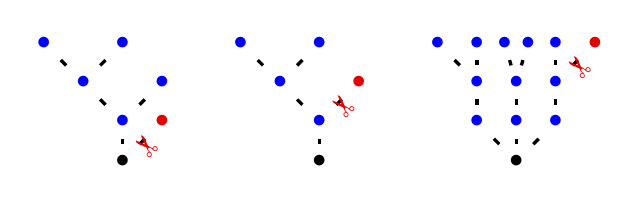
\begin{tikzpicture}[very thick, scale=0.25]
      \node (h1) at (4,0){$\bullet$};
      \node[blue] (h2) at (4,2){$\bullet$};
      \node[blue] (h3) at (2,4){$\bullet$};
      \node[blue] (h4) at (0,6){$\bullet$};
      \node[red!90!black] (h7) at (6,2){$\bullet$};
      \node[blue] (h5) at (4,6){$\bullet$};
      \node[blue] (h6) at (6,4){$\bullet$};
      \draw (h1) -- (h2) ;
      \draw (h2) -- (h3) ;
      \draw (h1) -- node[red!90!black,font=\small,sloped,
      shift={(0.01,-0.075)},rotate=90]{\textbf{\ding{34}}} (h7);
      \draw (h3) -- (h4) ;
      \draw (h3) -- (h5) ;
      \draw (h2) -- (h6);

      \node (h11) at (14,0){$\bullet$};
      \node[blue] (h12) at (14,2){$\bullet$};
      \node[blue] (h13) at (12,4){$\bullet$};
      \node[blue] (h14) at (10,6){$\bullet$};
      \node[blue] (h15) at (14,6){$\bullet$};
      \node[red!90!black] (h16) at (16,4){$\bullet$};
      \draw (h11) -- (h12) ;
      \draw (h12) -- (h13) ;
      \draw (h12) -- node[red!90!black,
      font=\small,sloped,shift={(0.01,-0.075)},
      rotate=90]{\textbf{\ding{34}}} (h16);
      \draw (h13) -- (h14) ;
      \draw (h13) -- (h15) ;
      
      \node (hn1) at (24,0){$\bullet$};
      \node[blue] (hn2) at (22,2) {$\bullet$};
      \node[blue] (hn3) at (22,4) {$\bullet$};
      \node[blue] (hn4) at (20,6){$\bullet$};
      \node[blue] (hn5) at (22,6){$\bullet$};
      \draw (hn1) -- (hn2) ;
      \draw (hn2) -- (hn3) ;
      \draw (hn3) -- (hn4) ;
      \draw (hn3) -- (hn5) ;
      \node [blue](hn2b) at (24,2) {$\bullet$};
      \node[blue] (hn3b) at (24,4) {$\bullet$};
      \node [blue](hn4b) at (23.4,6){$\bullet$};
      \node [blue](hn5b) at (24.6,6){$\bullet$};
      \draw (hn1) -- (hn2b) ;
      \draw (hn2b) -- (hn3b) ;
      \draw (hn3b) -- (hn4b) ;
      \draw (hn3b) -- (hn5b) ;
      \node [blue](hn2c) at (26,2) {$\bullet$};
      \node [blue](hn3c) at (26,4) {$\bullet$};
      \node [blue](hn4c) at (26,6){$\bullet$};
      \node [red!90!black] (hn5c) at (28,6){$\bullet$};
      \draw (hn1) -- (hn2c) ;
      \draw (hn2c) -- (hn3c) ;
      \draw (hn3c) -- (hn4c) ;
      \draw (hn3c) -- node[red!90!black,
      font=\small,sloped,shift={(0.01,-0.075)},
      rotate=90]{\textbf{\ding{34}}} (hn5c) ;
    \end{tikzpicture}

    \caption{Three successive states of a hydra in a battle,
      at time $t=0,1,2$\label{life1}}
    \label{fig:round}
  \end{figure}

  \begin{figure}[h]
    \centering
    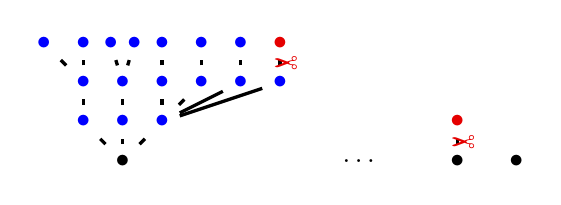
\begin{tikzpicture}[very thick, scale=0.25]
      \node (hn1) at (4,0){$\bullet$};
      \node[blue] (hn2) at (2,2) {$\bullet$};
      \node[blue] (hn3) at (2,4) {$\bullet$};
      \node[blue] (hn4) at (0,6){$\bullet$};
      \node[blue] (hn5) at (2,6){$\bullet$};
      \draw (hn1) -- (hn2) ;
      \draw (hn2) -- (hn3) ;
      \draw (hn3) -- (hn4) ;
      \draw (hn3) -- (hn5) ;
      \node [blue](hn2b) at (4,2) {$\bullet$};
      \node [blue](hn3b) at (4,4) {$\bullet$};
      \node [blue](hn4b) at (3.4,6){$\bullet$};
      \node [blue] (hn5b) at (4.6,6){$\bullet$};
      \draw (hn1) -- (hn2b) ;
      \draw (hn2b) -- (hn3b) ;
      \draw (hn3b) -- (hn4b) ;
      \draw (hn3b) -- (hn5b) ;
      \node [blue](hn2c) at (6,2) {$\bullet$};
      \node [blue](hn3c) at (6,4) {$\bullet$};
      \node [blue](hn4c) at (6,6){$\bullet$};
      \draw (hn1) -- (hn2c) ;
      \draw (hn2c) -- (hn3c) ;
      \draw (hn3c) -- (hn4c) ;
      \node [blue](hn3d) at (8,4) {$\bullet$};
      \draw (hn2c) -- (hn3d) ;
      \node [blue](hn4d) at (8,6) {$\bullet$};
      \draw (hn3d) -- (hn4d) ;
      
      \node [blue](hn3e) at (10,4) {$\bullet$};
      \draw (hn2c) -- (hn3e) ;
      \node [blue](hn4e) at (10,6) {$\bullet$};
      \draw (hn3e) -- (hn4e) ;

      \node [blue](hn3f) at (12,4) {$\bullet$};
      \draw (hn2c) -- (hn3f) ;
      \node [red!90!black](hn4f) at (12,6) {$\bullet$};
      \draw (hn3f) -- node[red!90!black,
      font=\small,sloped,shift={(0.01,-0.075)},
      rotate=90]{\textbf{\ding{34}}} (hn4f) ;

      \node at (16,0) {$\dots$} ;

      \node [black](hn4h) at (21,0) {$\bullet$};
      \node [red!90!black](hn4g) at (21,2) {$\bullet$};
      \draw (hn4h) -- node[red!90!black,
      font=\small,sloped,shift={(0.01,-0.075)},
      rotate=90]{\textbf{\ding{34}}} (hn4g) ;

      
      \node [black](hn4f) at (24,0) {$\bullet$};
      
    \end{tikzpicture}
    \caption{At $t=3,\dots,\textcolor{red}{x}-1,\textcolor{red}{x=?}$
      \label{life2}}
  \end{figure}
\end{frame}

%%%%%%%%%%%%%%%%%%%%%%%%%%%%%%%%%%%%%%%%%%%%

\begin{frame}
    \begin{block}{Mathematical formalization}
    
    \begin{itemize}
    \item   We associate a hydra to each ordinal \textcolor{mathcolor}{$\alpha<\epsilon_0$} (in Cantor normal form). For instance, the first hydra of our example is the image of \textcolor{mathcolor}{$\omega^{\omega^2+1}+1$}.
    \item A round (at time $t\in\mathbb{N}$) of a battle transforms an hydra associated with \textcolor{mathcolor}{$\alpha$} into the hydra associated with \textcolor{mathcolor}{$\canonseq{\alpha}{t+1}$}, the $t+1$-st element of the \emph{canonical sequence} of \textcolor{mathcolor}{$\alpha$}.
    \item We want to ``compute'' the length of sequences of the form 
      \textcolor{mathcolor}{$\langle \alpha_k=\alpha,\dots,\alpha_{i+1}=\canonseq{\alpha_i}{i+1},\dots, 1,0\rangle$}, where \textcolor{mathcolor}{$k\in\mathbb{N}$}.
      \item Such sequences are studied
      as \emph{$\alpha$-large sets of natural numbers}  in Ketonen \& Solovay's article
      \emph{Rapidly Growing {R}amsey Functions (1981)}.
    \end{itemize}
  \end{block}
\end{frame}

%%%%%%%%%%%%%%%%%%%%%%%%%%%%%%%%%%%%%%%% 

\begin{frame}
  \begin{block}{}
    \begin{itemize}
    \item Let \textcolor{mathcolor}{$0<\alpha<\epsilon_0$}, and \textcolor{mathcolor}{$i\in\mathbb{N}$}.
      The least index \textcolor{mathcolor}{$k$} such that \textcolor{mathcolor}{$\alpha_k=0$} is  \textcolor{mathcolor}{$H'_\alpha(i)$} where \textcolor{mathcolor}{$H'_\alpha$} is defined by transfinite induction over \textcolor{mathcolor}{$\alpha$}.

      \begin{align}
        H'_0(i) & = i\\
        H'_\alpha(i) &= H'_{(\canonseq{\alpha}{i+1})}(i)  \quad\textit{if $\alpha$ is a limit ordinal}\\
        H'_{\alpha}(i) &=H'_\beta(i+1) \quad\textit{if $\alpha=\beta+1$}
      \end{align}

    \end{itemize}
  \end{block}

  \begin{block}{}
    The \textcolor{mathcolor}{$H'_\alpha$} family,  is a variant of the  \emph{Hardy hierarchy of rapidly growing functions}. For instance, \textcolor{mathcolor}{$H'_{\omega^3+3}(0)\geq2^{2^N}$}, where \textcolor{mathcolor}{$N=2^{70}-1$}.

    {\color{lookcolor} Such functions defy common programming intuition: no test is possible, only proofs!}
  \end{block}
  
\end{frame}

%%%%%%%%%%%%%%%%%%%%%%%%%%%%%%%%%%%%%%%

\begin{frame}
  \frametitle{Ordinals in \coq}
  
  \begin{block}{}
    Ordinals less than {\color{mathcolor}$\omega^\omega, \epsilon_0,  \Gamma_0$} are represented as \emph{ordinal notations}: comparison, canonical sequences, partition limit/successors/zero ordinals are implemented by certified functions, allowing the user to write proofs by computation.

    \begin{footnotesize}
      \inputsnippets{./ONDef}

      \inputsnippets{../E0_Ex42}
    \end{footnotesize}

    
    
  \end{block}
\end{frame}

%%%%%%%%%%%%%%%%%%%%%%%%%%%%%%%%%%%%%%%%%%%%

\begin{frame}
  \begin{block}{}
    The functions \textcolor{mathcolor}{$H'_\alpha\;(\alpha< \epsilon_0)$} are implemented with \textcolor{plugincolor}{coq-equations}.
    \vspace{5pt}
    \begin{footnotesize}
      \inputsnippets{../Hprime_HprimeDef}   
    \end{footnotesize}
    
  \end{block}

  \begin{block}{}
    Using combinatorial lemmas by  K. \& S., we prove (by mutual  transfinite induction on \textcolor{mathcolor}{$\alpha$}):
    \begin{quote}
      \begin{itemize}
      \item \textcolor{mathcolor}{$H'_\alpha$} is strictly monotonous
      \item \textcolor{mathcolor}{$\forall i, i \leq H'_\alpha(i)$}
      \item   If \textcolor{mathcolor}{$\beta<\alpha$}, then \textcolor{mathcolor}{$H'_\alpha(i)>H'_\beta(i)$} for all but a finite number of $i$ (we say that \textcolor{mathcolor}{$H'_\alpha$}
        \emph{dominates} \textcolor{mathcolor}{$H_\beta$}).
      \end{itemize}
    \end{quote}

  \end{block}
\end{frame}

%%%%%%%%%%%%%%%%%%%%%%%%%%%%%%%%%%%%%%%%%%%% 

\begin{frame}
  \begin{block}{Theorem}
    For any   \textcolor{mathcolor}{$\alpha\geq\omega^\omega$} the function \textcolor{mathcolor}{$H'_\alpha$} is not primitive recursive.
  \end{block}
  
  \begin{block}{}
    {\color{coqstylecolor}
      \begin{itemize}
      \item \emph{In order to prove this theorem, we chose to host and  maintain under \community Russel O'Connor's library \textcolor{plugincolor}{goedel}, which contains a formalization of primitive recursive functions.}
        
      \item    \emph{The interest of O'Connor's contribution led us to write a chapter on primitive recursive functions, with [counter-]examples and exercices.}

      \item \emph{Proving formally that a given function is not primitive recursive is a nice example of application of a complex (mutually recursive, dependently typed) induction principle. You have to take into account the set of PR functions of any arity.}
        
      \end{itemize}
    }
  \end{block}
\end{frame}

%%%%%%%%%%%%%%%%%%%%%%%%%%%%%%%%%%%%%%%%%

\begin{frame}
  
  \begin{scriptsize}
    \inputsnippets{./SchemePrimRecInda}
  \end{scriptsize}
\end{frame}

%%%%%%%%%%%%%%%%%%%%%%%%%%%%%%%%%%%%%%%%%%%

\begin{frame}
  \begin{block}{}
    Using  \texttt{PrimRec\_PrimRecs\_ind}, we prove the following lemma:
    
    \begin{quote}
      For any \textcolor{mathcolor}{$n$}, and any primitive recursive function \textcolor{mathcolor}{$f$} of  arity \textcolor{mathcolor}{$n$}, there exists some natural number \textcolor{mathcolor}{$q$} such that the following inequality holds:
      {\color{mathcolor}
        \[
          \forall x_1,\dots,x_n, 
          f(x_1,\dots,\,x_n)\leq\textrm{Ack}(q,\textrm{max}(x_1,\dots,x_n))
        \]}
    \end{quote}
  \end{block}


  \begin{block}{}

    Instantiating with \textcolor{mathcolor}{$n=1$}, we obtain:

    \begin{quote}
      If \textcolor{mathcolor}{$H'_{\omega^\omega}$} were primitive recursive, there would exists some \textcolor{mathcolor}{$q$} such that, for any \textcolor{mathcolor}{$k$}, \textcolor{mathcolor}{$H'_{\omega^\omega}(k) \leq\textrm{Ack}(q,k)$}, which is false.
    \end{quote}
    
  \end{block}
\end{frame}
%%%%%%%%%%%%%%%%%%%%%%%%%%%%%%%%%%%%%%%%%%
\section{Project Organization}
\begin{frame}
  \frametitle{Project  Organization}
  \begin{itemize}
  \item Integration with \community
  \item Documentation with \alectr
  \item Package dependencies
  \item Continuous integration
  \end{itemize}
\end{frame}

  %%%%%%%%%%%%%%%%%%%%%%%%%%%%%%%%%%%%%%%%%
  \begin{frame}
    \frametitle{\community}
    \begin{block}{}
      \community is an informal organization that aims to maintain interesting open source \coq projects and facilitate collaboration among Coq users on documentation, tooling, etc.
      \begin{itemize}
      \item Created in 2018,  run by volunteer Coq users on GitHub
      \item At present, over than 50 projects, maintained by over than 30 volunteers
      \item Some packages were unmaintained before their integration to \community. According to their scientific or historical interest, we decided to revive them.
        \item After their transfer, packages may be the object of large changes  and refactorings.
      \end{itemize}
    \end{block}
  \end{frame}

%%%%%%%%%%%%%%%%%%%%%%%%%%%%%%%%%%%%%%%%% 
\section{Presenting proofs with \alectr}
\begin{frame}
  \frametitle{Presenting proofs with \alectr}
  \begin{block}{}
    \begin{itemize}
    \item The order in which \coq code, goals and answers are presented in the book is determined by the difficulty of the mathematical examples, or the assumed level in \coq of the reader, not by the structure of the libraries.
    \item
      \emph{\coq libraries contain \emph{snippet declarations} which are converted during the compilation of the book into \LaTeX\xspace blocks which are inserted into the book.}

    \item {\color{lookcolor} \emph{Note that our build system guarantees that the accompanying book is always up-to-date and consistent with the \coq code.}}
    \end{itemize}
  \end{block}
\end{frame}

%%%%%%%%%%%%%%%%%%%%%%%%%%%%%%%%%%%%%%%%% 

\begin{frame}[fragile]
\begin{alltt}
{\color{lightblue}{(* begin snippet Ex42a:: no-out *)}}
Example Ex42: omega + 42 + omega^2 = omega^2. 
{\color{lightblue}{(* end snippet Ex42a *)}}
Proof.
  {\color{lightblue}{(* begin snippet Ex42b *)}}
  assert (HAP:= AP_phi0 2). {\color{lightblue}{(* .no-out *)}}
  elim  HAP; intros _ H0; apply H0; clear H0. 
  {\color{lightblue}{(* end snippet Ex42b *)}}
  {\color{lightblue}{(* begin snippet Ex42d *)}}
  Check AP_plus_closed. {\color{lightblue}{(* .unfold .no-goals *)}}
  {\color{lightblue}{(* end snippet Ex42d *)}}
   {\color{lightblue}{(* begin snippet Ex42c *)}}
  assert (Hlt: omega < omega^2) by 
      (rewrite omega_eqn; apply phi0_mono, finite_mono;
        auto with arith).
 {\color{lightblue}{ (* end  snippet Ex42c *)}}
\end{alltt}
\end{frame}

%%%%%%%%%%%%%%%%%%%%%%%%%%%%%%%%%%%%%%%%%%

\begin{frame}
  \begin{small}
    
     \inputsnippets{../Schutte_Ex42a}   

     By definition of additive principal ordinals, 
    it suffices to prove the inequality $\omega+42< \phi_0(2)$.

    \inputsnippets{../Schutte_Ex42b}
    By Lemma \textit{AP\_plus\_closed}, it suffices to prove  $\omega<\omega^2$ and $42<\omega^2$.
  \end{small}

\end{frame}

\begin{frame}
  \begin{small}
    \inputsnippets{
      ../Schutte_Ex42c, ../Schutte_Ex42d, ../Schutte_Ex42e}
  \end{small}
  
\end{frame}

%%%%%%%%%%%%%%%%%%%%%%%%%%%%%%%%%%%%%%%%

\begin{frame}
    
  \begin{block}{Remarks}
    \begin{itemize}
    \item We could write the book, because we are also the maintainers of the cited \coq source, and could insert the snippet instructions in the \texttt{.v} files. \textcolor{lookcolor}{But what about commenting interesting code from other people (\emph{e.g.},
        \gaia) ?}
    \item The same  piece of \coq code may be used in several documents, with different styles (book, beamer), and thus
      different filters (hiding or showing subgoals, hypotheses, etc.).
      
    \end{itemize}
  \end{block}

  \begin{block}{To do ?}
    Define a language for
    \begin{itemize}
    \item Searching sentences in any \coq file,
    \item Applying filters in order to generate as many snippets as needed.
    \end{itemize}
  \end{block}
\end{frame}
%%%%%%%%%%%%%%%%%%%%%%%%%%%%%%%%%%%%%%%%%%

\begin{frame}
  \frametitle{Package organization and dependencies}
  
\begin{figure}[ht]
\centering
\scalebox{0.7}{
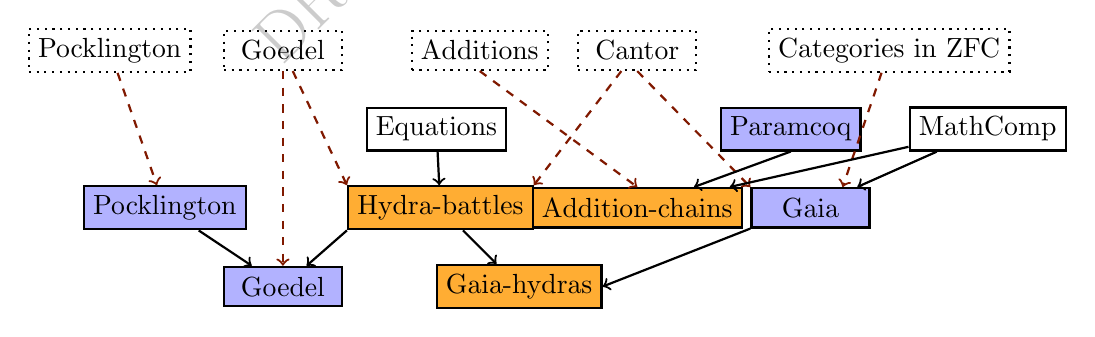
\begin{tikzpicture}[thick]

\begin{scope}[xshift=-6cm]
\node[rectangle, dotted,draw=black,minimum height=0.5cm,minimum width=1.5cm] (goedel) { Goedel };
\node[rectangle, dotted,draw=black,minimum height=0.5cm,minimum width=1.5cm,left of=goedel, node distance=2.2cm] (pock) { Pocklington };
\node[rectangle, dotted,draw=black,minimum height=0.5cm,minimum width=1.5cm,right of=goedel, node distance=2.5cm] (additions) { Additions };
\node[rectangle, dotted,draw=black,minimum height=0.5cm,minimum width=1.5cm,right of=additions, node distance=2cm] (cantor) { Cantor };

\node[rectangle, dotted,draw=black,minimum height=0.5cm,minimum width=1.5cm,right of=cantor, node distance=3.2cm] (cats) { Categories in ZFC };
\end{scope}

\begin{scope}[yshift=-1cm,xshift=0.45cm]
  \node[rectangle, draw=black,fill=blue!30,minimum height=0.5cm,minimum width=1.5cm] (paramcoq) { Paramcoq };
\node[rectangle, draw=black,minimum height=0.5cm,minimum width=1.5cm,right of=paramcoq, node distance=2.5cm] (mathcomp) { MathComp };
\node[rectangle, draw=black,minimum height=0.5cm,minimum width=1.5cm,node distance=2cm,left of=paramcoq, node distance=4.5cm] (equations) { Equations };
\end{scope}

\begin{scope}[yshift=-2cm,xshift=-4cm]
\node[rectangle, draw=black,fill=orange!80,minimum height=0.5cm,minimum width=1.5cm] (hydras) { Hydra-battles };
\node[rectangle, draw=black,fill=blue!30,minimum height=0.5cm,minimum width=1.5cm,left of=hydras, node distance=3.5cm] (pockcc) { Pocklington };
\node[rectangle, draw=black,fill=orange!80,minimum height=0.5cm,minimum width=1.5cm,right of=hydras, node distance=2.5cm] (chains) { Addition-chains };
\node[rectangle, draw=black,fill=blue!30,minimum height=0.5cm,minimum width=1.5cm,right of=chains, node distance=2.2cm] (gaia) { Gaia };
\end{scope}

\begin{scope}[yshift=-3cm,xshift=-6cm]
 \node[rectangle, draw=black,fill=blue!30,minimum height=0.5cm,minimum width=1.5cm] (goedelcc) { Goedel };
 \node[rectangle, draw=black,fill=orange!80,minimum height=0.5cm,minimum width=1.5cm,right of=goedelcc, node distance=3cm] (gaiahydras) { Gaia-hydras };
\end{scope}

\draw[lookcolor,->,dashed] (additions.south) -- (chains.north) ;
\draw[lookcolor,->,dashed] (goedel) -- (goedelcc) ;
\draw[lookcolor,->,dashed] (goedel) -- (hydras.north west) ;
\draw[lookcolor,->,dashed] (cantor) -- (hydras.north east) ;
\draw[lookcolor,->,dashed] (cantor.south) -- (gaia.north west) ;
\draw[lookcolor,->,dashed] (pock) -- (pockcc) ;
\draw[lookcolor,->,dashed] ([xshift=2.1cm]cats) -- (gaia) ;

\draw[->] (hydras) -- (gaiahydras) ;
\draw[->] (hydras.south west) -- (goedelcc) ;
\draw[->] (gaia.south west) -- (gaiahydras.east) ;

\draw[->] (equations) -- (hydras) ;
\draw[->] (mathcomp) -- (gaia) ;
\draw[->] (mathcomp) -- (chains) ;
\draw[->] (paramcoq.south) -- (chains) ;
\draw[->] (pockcc) -- (goedelcc) ;
\end{tikzpicture}
}
\caption{\textcolor{lookcolor}{Genealogy} and dependencies for \Hydras packages.}
 %Dotted boxes represent historical Coq contributions, while regular boxes represent maintained \coq packages. Orange packages are maintained in the \Hydras GitHub repository, while blue packages are maintained in other \community repositories. Dotted lines represent \coq code ancestry, while regular lines represent direct code dependencies.}
  \label{fig:genealogy}
\end{figure}

%%%% TODO : Resize  !
{\scriptsize
\begin{table}[ht]
\centering
\scriptsize
\begin{tabular}{llllrr}
\hline
\textbf{Package name} &  \textbf{Version} & \textbf{Spec LOC} & \textbf{Proof LOC}\\
\hline
Pocklington & \texttt{8.12.0} & 825 & 3,798 \\
Goedel  & \texttt{8.13.0} & 2,799 & 10,762 \\
Gaia &  \texttt{1.12} & 28,850 & 124,839 \\
Hydra-battles & \texttt{0.5} & 14,368 & 48,385 \\
Addition-chains & \texttt{0.5} & 1,961 & 2,210 \\
Gaia-hydras &  \texttt{0.5} & 81 & 177 \\
\hline
\end{tabular}
\caption{\scriptsize Current numbers of lines of code for packages in the \Hydras galaxy.}
\label{tbl:loc}
\end{table}}
\end{frame}
%%%%%%%%%%%%%%%%%%%%%%%%%%%%%%%%%%%%%%%%%%

% \begin{frame}
%   \TODO{}{maintenance, CI/CD,  etc.   (several slides).}
% \end{frame}

%%%%%%%%%%%%%%%%%%%%%%%%%%%%%%%%%%%%%%% 

\begin{frame}
  \frametitle{Conclusion and perspectives}
  \begin{block}{}
    \begin{itemize}
    \item \Hydras wants to be a connection between scientific litterature and proof assistant technology:
      \begin{itemize}
      \item For the mathematician, it gives a concrete view of the mathematical contents: full proofs, examples, computable functions whenever possible, etc.
        \item  For the \coq learner, it provides a consistent set of examples,
allowing to present and compare various formalization and proving techniques.
      \end{itemize}
    \end{itemize}
  \end{block}
  \end{frame}

%%%%%%%%%%%%%%%%%%%%%%%%%%%%%%%%%%%%%%%%%%%%%%

\begin{frame}[fragile]
  \frametitle{Perspectives}
  \begin{block}{Library on ordinals}
    There exist already \coq libraries which formalize ordinal numbers.
    \begin{itemize}
    \item \gaia (José Grimm) : Formalization of Bourbaki's Elements of Mathematics. {\color{lookcolor}\emph{This library uses an ordinal representation compatible with ours. It is  written in SSReflect/Mathcomp, and is also maintained in \community}.}
    \item A formalization by Minki Cho, using a different representation.
{\color{darkorange}
\begin{verbatim}
Inductive Ord.t :=
| Ord.build: 
    forall (A: Type), (A -> Ord.t) -> Ord.t.
\end{verbatim}
}  
    \end{itemize}

    Both libraries contain set-theoretical results about larger ordinals than ours. Having a library containing both our combinatorial results (large sets and rapidly growing functions) and mathematical definitions of ordinals would be an interesting project.
  \end{block}
\end{frame}




%%%%%%%%%%%%%%%%%%%%%%%%%%%%%%%%%%%%%%%%%%%

\begin{frame}
  \frametitle{More TODOs}
  \begin{block}{}
    \begin{itemize}
    \item More results about hyper-complexity and fast growing functions
    \item New toolchain for \alectr
    \item More proof and specification patterns
    \item etc.
    \item \Hydras and \community are on GitHub. Please contribute!
      \begin{itemize}
      \item New chapters
      \item Any correction or improvement (text and/or proofs)
        
      \end{itemize}
    \end{itemize}
    
  \end{block}
  
\end{frame}


\end{document}

